\clearpage\section{Labs}\begin{Lab}

\begin{exe} {Networking Basics}

	\subsection*{Adding A New IP Address}
   We will begin by documenting our network configuration. 
	There are several tools your distribution could use

      \begin{enumerate}
         \item
		 Open a terminal or a PuTTY session. Use the 
		      \textbf{ip} command
		      to view your interfaces and addresses.
		      Save it to a file for later reference.
		      \begin{raw}
$ ip a
1: lo: <LOOPBACK,UP,LOWER_UP> mtu 65536 qdisc noqueue state UNKNOWN group default qlen 1000
    link/loopback 00:00:00:00:00:00 brd 00:00:00:00:00:00
    inet 127.0.0.1/8 scope host lo
       valid_lft forever preferred_lft forever
    inet6 ::1/128 scope host
       valid_lft forever preferred_lft forever
2: eth0: <BROADCAST,MULTICAST,UP,LOWER_UP> mtu 9001 qdisc mq state UP group default qlen 1000
    link/ether 06:04:be:c0:bf:7c brd ff:ff:ff:ff:ff:ff
    inet 172.31.21.106/20 brd 172.31.31.255 scope global dynamic eth0
       valid_lft 2225sec preferred_lft 2225sec
    inet6 fe80::404:beff:fec0:bf7c/64 scope link
       valid_lft forever preferred_lft forever

$ ip a > ~/before.txt
		      \end{raw}

         \item
		 Determine if \verb:systemd-networkd: is running. As
		      there are many \texttt{possible} tools, it may
		      or may not be running. Following shows an 
		      example of it not running. If your system is using
		      the daemon and it is active, find your config files, 
		      probably under \file{/etc/systemd/network/}. Review
		      the contents.
		      \begin{raw}
$ systemctl status systemd-networkd
● systemd-networkd.service - Network Service
   Loaded: loaded (/lib/systemd/system/systemd-networkd.service; disabled; vendo
   Active: inactive (dead)
     Docs: man:systemd-networkd.service(8)
		      \end{raw}

	 \item
		 Determine if \verb:Network Mangager: is 
		      configuring you network. Again, you system
		      may be different. Once you find a profile in
		      use run the command again to view the details.
		      \begin{raw}
$ nmcli connection show 
NAME                      UUID                                  TYPE    DE
WorkNet                   235d15bb-8d60-4889-86a2-c5787c46dea8  wifi    wl
....		      
		      
$ nmcli con show WorkNet
connection.id:                          WorkNet
connection.uuid:                        235d15bb-8d60-4889-86a2-c5787c46dea8
connection.stable-id:                   --
connection.type:                        802-11-wireless
connection.interface-name:              --
connection.autoconnect:                 yes
connection.autoconnect-priority:        0
....
		      \end{raw}
	      \item
		      View flat file configuration. Your file 
		      name may vary depending on your distribution.
		      View the file contents as you find them. Note 
		      the prompts in the commands indicate which 
		      distribution you may find the file.
\begin{raw}
ubuntu$ ls -l /etc/network/interfaces

ubuntu$ ls -l /etc/network/interfaces.d/


redhat$ ls -l /etc/sysconfig/network-scripts/

\end{raw}
         \item
		 Use the \textbf{ip} command to add a new IP 
		      Address to your primary interface. Your
		      interface name may be different. Typically
		      the interface listed after \verb:lo: in the
		      \textbf{ip} output is your primary. Add the
		      \verb:10.1.2.3: address. We will need to use
		      the \textbf{sudo} command.
\begin{raw}
$ sudo ip addr add 10.1.2.3 dev wlp1s0
\end{raw}
	      \item
		      Use \textbf{ping} to test connection to the
		      new address.
		      \begin{raw}
$ ping -c3 10.1.2.3
PING 10.1.2.3 (10.1.2.3) 56(84) bytes of data.
64 bytes from 10.1.2.3: icmp_seq=1 ttl=64 time=0.049 ms
64 bytes from 10.1.2.3: icmp_seq=2 ttl=64 time=0.155 ms
64 bytes from 10.1.2.3: icmp_seq=3 ttl=64 time=0.116 ms

--- 10.1.2.3 ping statistics ---
3 packets transmitted, 3 received, 0% packet loss, time 2037ms
rtt min/avg/max/mdev = 0.049/0.106/0.155/0.045 ms
		      \end{raw}
	      \item
		      View the \textbf{ip} details of the interface.
		      Verify the new IP address has been added. Note
		      it is not an alias, but an equal IP as the previous.
		      \begin{raw}
$ sudo ip addr show wlp1s0
2: wlp1s0: <BROADCAST,MULTICAST,UP,LOWER_UP> mtu 900 qdisc mq state UP 
	group default qlen 1000
    link/ether 94:65:9c:7b:cd:a7 brd ff:ff:ff:ff:ff:ff
    inet 172.30.9.192/21 brd 172.30.15.255 scope global dynamic 
	noprefixroute wlp1s0
       valid_lft 18306sec preferred_lft 18306sec
    inet 10.1.2.3/32 scope global wlp1s0
       valid_lft forever preferred_lft forever
		      \end{raw}
	      \item
		      View the route information with \textbf{ip route}.
		      Note your information will not match the exact 
		      output as your network is different. Look for
		      a route for your new IP adress. It may not be there.
		      \begin{raw}
$ ip route
default via 172.30.8.1 dev wlp1s0 proto dhcp metric 600 
10.0.3.0/24 dev lxcbr0 proto kernel scope link src 10.0.3.1 linkdown 
169.254.0.0/16 dev virbr1 scope link metric 1000 linkdown 
172.17.0.0/16 dev docker0 proto kernel scope link src 172.17.0.1 linkdown 
172.30.8.0/21 dev wlp1s0 proto kernel scope link src 172.30.9.192 metric 600
		      \end{raw}
		      
	      \item
		      Add a new route to \verb:192.0.2.1: via \verb:10.1.2.3:
		      and verify it it is shown in the \textbf{ip route}
		      output. Your interface may be different. View the
		      new entry to the route table.
		      \begin{raw}
$ sudo ip route add 192.0.2.1 via 10.1.2.3 dev wlp1s0

$ sudo ip route
default via 172.30.8.1 dev wlp1s0 proto dhcp metric 600 
10.0.3.0/24 dev lxcbr0 proto kernel scope link src 10.0.3.1 linkdown 
169.254.0.0/16 dev virbr1 scope link metric 1000 linkdown 
172.17.0.0/16 dev docker0 proto kernel scope link src 172.17.0.1 linkdown 
172.30.8.0/21 dev wlp1s0 proto kernel scope link src 172.30.9.192 metric 600 
192.0.2.1 via 10.1.2.3 dev wlp1s0 
....
		      \end{raw}
	      \item
		      Use the \textbf{ifconfig -a} command to view
		      your network settings.  Do you see the new,
		      working IP Address?
		      \begin{raw}
$ sudo ifconfig -a
.....
wlp1s0: flags=4163<UP,BROADCAST,RUNNING,MULTICAST>  mtu 900
        inet 172.30.9.192  netmask 255.255.248.0  broadcast 172.30.15.255
        ether 94:65:9c:7b:cd:a7  txqueuelen 1000  (Ethernet)
        RX packets 217530  bytes 154308545 (154.3 MB)
        RX errors 0  dropped 0  overruns 0  frame 0
        TX packets 87257  bytes 22436095 (22.4 MB)
        TX errors 0  dropped 0 overruns 0  carrier 0  collisions 0
		      \end{raw}
(So, no. It's not there.)


	      \item
		      Remove the IP address. After it has been removed, 
		      check to see if the routes have been removed as 
		      well. If not, remove it.
		      \begin{raw}
$ sudo ip addr del 10.1.2.3/32 dev wlp1s0 


$ sudo ip route
default via 172.30.8.1 dev wlp1s0 proto dhcp metric 600 
10.0.3.0/24 dev lxcbr0 proto kernel scope link src 10.0.3.1 linkdown 
10.1.2.3 dev wlp1s0 proto kernel scope link src 10.1.2.3 metric 600 
169.254.0.0/16 dev virbr1 scope link metric 1000 linkdown 
172.17.0.0/16 dev docker0 proto kernel scope link src 172.17.0.1 linkdown 
172.30.8.0/21 dev wlp1s0 proto kernel scope link src 172.30.9.192 metric 600 
192.0.2.1 via 10.1.2.3 dev wlp1s0 
192.168.99.0/24 dev virbr1 proto kernel scope link src 192.168.99.1 linkdown 
192.168.123.0/24 dev virbr0 proto kernel scope link src 192.168.123.1 linkdown 


$ sudo ip route del 10.1.2.3 dev wlp1s0
		      \end{raw}

      \end{enumerate}

	\subsection*{Changing Parameters}
   In this section we will change the \verb:MTU: and view
	the differences in performance. You can test between 
	two VMs or instances, or between yourself and another
	in class. For ease of use we will test against ourselves.
	Be aware that other network traffic can
	skew results. You may want to test mutliple times.
	Also, some wifi drivers have a lower limit allowed,
	cloud providers like AWS and GCE set their MTU much
	higher automatically. Your
	interface particulars may be different. 
	\begin{enumerate}
		\item Verify the MTU of your primary interface 
			is \verb:1500:.
			\begin{raw}
$ $ sudo ip addr show wlp1s0 
2: wlp1s0: <BROADCAST,MULTICAST,UP,LOWER_UP> mtu 1500 qdisc mq 
  state UP group default qlen 1000
    link/ether 94:65:9c:7b:cd:a7 brd ff:ff:ff:ff:ff:ff
    inet 172.30.9.192/21 brd 172.30.15.255 scope global dynamic 
  noprefixroute wlp1s0
       valid_lft 40986sec preferred_lft 40986sec

			\end{raw}
		\item Install the Flexible IO, or \textbf{fio}, package.
			We will use this command to generate a 
			known amount of traffic. Ubuntu users can use
			the \textbf{apt-get} command, and Red Hat users
			can use the \textbf{yum} or \textbf{dnf} 
			command.
			\begin{raw}
ubuntu$ sudo apt-get update ; sudo apt-get -y install fio

redhat$ sudo yum -y install fio
			\end{raw}
		\item
			Use \textbf{fio} to test network transfer. 
			Copy and paste the summary information to 
			a temporary file or notepad. If you are not
			familiar with \textbf{fio} you can find 
			several other example files in the same 
			directory. The command will run for about
			two minutes, with a summary at the end. Go
			slow the first time and view all the summary.
			\begin{raw}
$ fio /usr/share/doc/fio/examples/netio.fio
....
Run status group 0 (all jobs):
   READ: bw=5749Mibit/s (6029Mbit/s), 5749Mibit/s-5749Mibit/s (6029Mbit/s-6029Mbit/s), io=99.0GiB (107GB), run=142482-142482msec
  WRITE: bw=5750Mibit/s (6029Mbit/s), 5750Mibit/s-5750Mibit/s (6029Mbit/s-6029Mbit/s), io=100GiB (107GB), run=142471-142471msec
			\end{raw}

		\item
			Change the \verb:MTU: and run the test again.
			Note the performance change as the \verb:MTU:
			Changes. Set it as low as the driver allows,
			such as 500, and as high as the driver allows,
			such as 9000. When testing to a remote node
			via a switch you may notice an even greater
			amount of difference in performance.
			\begin{raw}
$ sudo ip link set dev wlp1s0 mtu 500 
			\end{raw}
	\end{enumerate}

\subsection*{Testing Name Services}
    In this section we will test that we can resolve
    IP addresses, both forward and reverse lookups.
	        \begin{enumerate}
                \item 
			Use the \textbf{host} command to
				view the IP information for
				\verb:Linux.com:.
				\begin{raw}
$ host Linux.com
Linux.com has address 151.101.65.5
Linux.com has address 151.101.129.5
Linux.com has address 151.101.193.5
Linux.com has address 151.101.1.5
Linux.com mail is handled by 10 smtp2.linuxfoundation.org.
Linux.com mail is handled by 10 smtp1.linuxfoundation.org.
				\end{raw}

			\item
				Compare the output with what
				you can see using the \textbf{nslookup} 
				command.
				\begin{raw}
$ nslookup Linux.com
Server:		127.0.0.53
Address:	127.0.0.53#53

Non-authoritative answer:
Name:	Linux.com
Address: 151.101.1.5
Name:	Linux.com
Address: 151.101.193.5
Name:	Linux.com
Address: 151.101.129.5
Name:	Linux.com
Address: 151.101.65.5

				\end{raw}

			\item
				Use the \textbf{dig} command to view
				all the DNS information about
				\verb:Linux.com:.
				\begin{raw}
$ dig Linux.com

; <<>> DiG 9.11.3-1ubuntu1.8-Ubuntu <<>> Linux.com
;; global options: +cmd
;; Got answer:
;; ->>HEADER<<- opcode: QUERY, status: NOERROR, id: 15396
;; flags: qr rd ra; QUERY: 1, ANSWER: 4, AUTHORITY: 0, ADDITIONAL: 1

;; OPT PSEUDOSECTION:
; EDNS: version: 0, flags:; udp: 65494
;; QUESTION SECTION:
;Linux.com.			IN	A

;; ANSWER SECTION:
Linux.com.		10	IN	A	151.101.193.5
Linux.com.		10	IN	A	151.101.129.5
Linux.com.		10	IN	A	151.101.65.5
Linux.com.		10	IN	A	151.101.1.5

;; Query time: 0 msec
;; SERVER: 127.0.0.53#53(127.0.0.53)
;; WHEN: Wed Aug 21 05:04:22 UTC 2019
;; MSG SIZE  rcvd: 102
				\end{raw}
			\item
				View the name servers(NS) and mail server(MX)
				for the \verb:Linux.com: network. The output
				to the commands is not shown below. You
				should see a couple entries for each.
				\begin{raw}
$ $ dig -t NS Linux.com
....

$dig -t MX Linux.com
....

				\end{raw}

			\item
				Choose an IP from the output and use 
				\textbf{dig} to resolve the name using the
				IP address. Note the \verb:PTR: record does
				not show a name.
				\begin{raw}
$ dig -X 151.101.193.5

; <<>> DiG 9.11.3-1ubuntu1.8-Ubuntu <<>> -x 151.101.193.5
;; global options: +cmd
;; Got answer:
;; ->>HEADER<<- opcode: QUERY, status: NXDOMAIN, id: 31490
;; flags: qr rd ra; QUERY: 1, ANSWER: 0, AUTHORITY: 0, ADDITIONAL: 1

;; OPT PSEUDOSECTION:
; EDNS: version: 0, flags:; udp: 65494
;; QUESTION SECTION:
;5.193.101.151.in-addr.arpa.	IN	PTR

;; Query time: 23 msec
;; SERVER: 127.0.0.53#53(127.0.0.53)
;; WHEN: Wed Aug 21 05:09:14 UTC 2019
;; MSG SIZE  rcvd: 55
				\end{raw}
			\item
				Check a DNS server for Google. Find the
				name it resolves to:
				\begin{raw}
$ dig -x 4.2.2.2
.....
2.2.2.4.in-addr.arpa.	60	IN	PTR	b.resolvers.Level3.net.
....
				\end{raw}

			\item
				Check your primary interface IP and determine
				if a name is known. Check your route gateway
				as well. By now you should be able to find 
				the IP and use \textbf{dig}, with being
				shown the command. A blank prompt is shown
				if you want to write in your own command.
				\begin{raw}
$
				\end{raw}

        \end{enumerate}



	        \subsection*{Monitoring Traffic}
		In this section we will use commands to
		view the network traffic.
        \begin{enumerate}
		\item Use \textbf{tcpdump} to view traffic
			on your \verb:lo: interface. Use
			\textbf{Ctrl-c} to stop the command.
			Then view traffic on your primary
			interface. Use the \textbf{ip} 
			command to find your primary interface.
			\begin{raw}
$ sudo tcpdump -i wlp1s0
....
05:13:19.469554 IP 12.235.16.3.54146 > ip-172-31-21-106.us-west-2.compute.internal.ssh: Flags [P.], seq 1333:1369, ack 2051348, win 2140, options [nop,nop,TS val 3815739841 ecr 397169965], length 36
....
			\end{raw}
		\item
			Use a filter to narrow down traffic to
			only port 80, if there is any.
			\begin{raw}
$ sudo tcpdump tcp port 80 -i eth0
tcpdump: verbose output suppressed, use -v or -vv for full protocol decode
listening on eth0, link-type EN10MB (Ethernet), capture size 262144 bytes
^C
0 packets captured
0 packets received by filter
0 packets dropped by kernel
			\end{raw}
		\item
			Use \textbf{tcpdump} to save traffic
			to a \verb:pcap: file. Let the command
			run for a moment, then interrupt with
			\textbf{Ctrl-c}. If asked, answer yes
			to any questions.
			\begin{raw}
$ sudo tcpdump -i eth0 -w traffic.out.pcap
			\end{raw}
		\item
			Install \textbf{Wireshark}. 
			\begin{raw}
ubunut$ sudo apt-get install -y wireshark

redhat$ sudo yum -y install wireshark
			\end{raw}

		\item
			Use \textbf{sudo} to start
			\textbf{wireshark}. Be aware you
			may need to use the \textbf{ssh -X}
			command or other configuration in 
			PuTTY for the display to export back 
			to your local system, if connecting 
			to a remote node. Select \verb:any:
			interface to begin collecting packets.
			\begin{raw}
$ sudo wireshark
			\end{raw}
   \begin{figure}[H]
   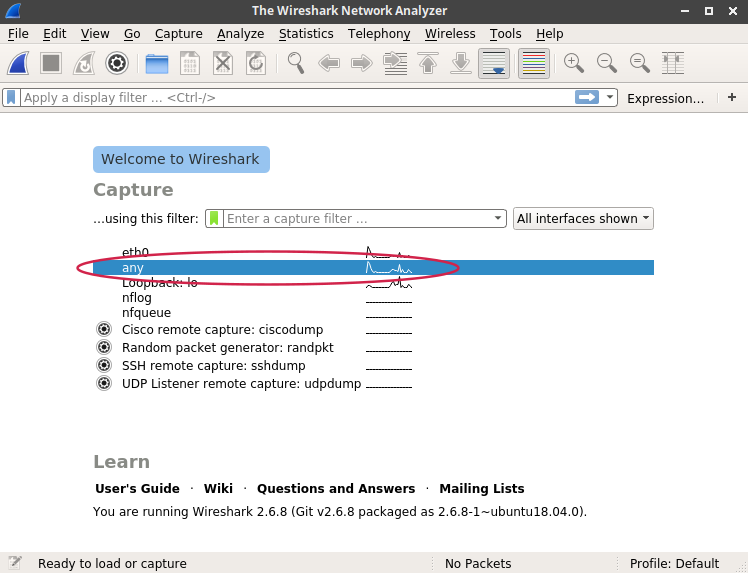
\includegraphics[width=6.4in]{IMAGES/wireshark2}
   \caption{Capture Traffic on Any Interface}
      \end{figure}

		\item
			The red square allows you to stop gathering
			packets. View some of the display filters by
			typing in the box, or selecting the 
			\verb:Expression: drop down.

		\item
			After you stop collecting traffic you can go
			under \textbf{File} then \textbf{Open} and
			open the \file{traffic.out.pcap} file you
			created using \textbf{tcpdump}. Select a 
			packet and explore the packet.
   \begin{figure}[H]
   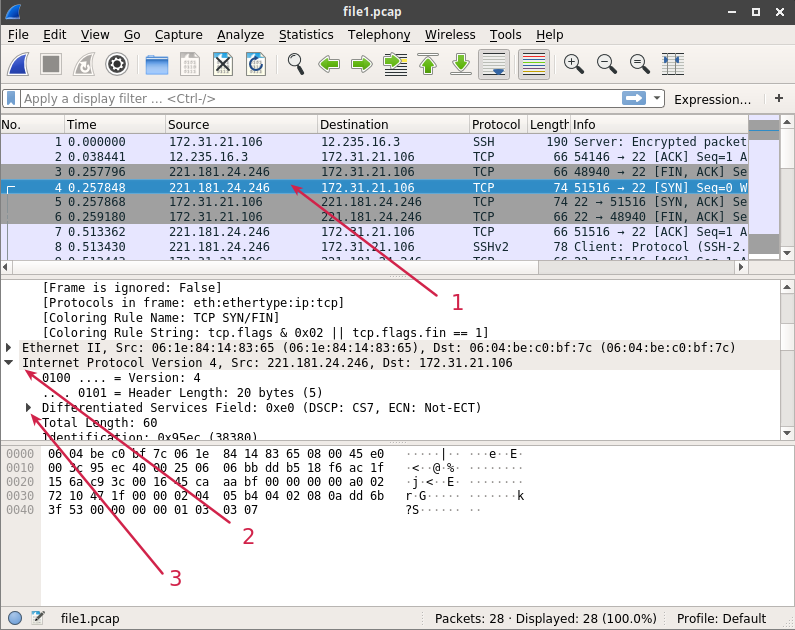
\includegraphics[width=6.4in]{IMAGES/wireshark3}
   \caption{View A PCAP File}
      \end{figure}

		\item 
			Experiment with \textbf{wireshark} as 
			time allows. Work through the menus at
			the top and see the various tools and
			features available.
        \end{enumerate}

\end{exe}
\end{Lab}
